\section{Introduction}
\label{sec:intro}

% Reinforcement learning has previously been used to solve a number of different games such as Chess\footnote{\href{https://arxiv.org/pdf/1712.01815.pdf}{Mastering Chess and Shogi by Self-Play with a General Reinforcement Learning Algorithm}} and Go\footnote{\href{https://www.nature.com/articles/nature24270.epdf}{Mastering the game of Go without human knowledge}}, both of which are zero sum games. Reinforcement learning has excelled at playing Go, where the number of possible moves are so many that a traditional heuristic is not sufficient to solve the problem successfully. These games only contain two players, whereas a game like Dota II is 5 vs. 5 game. That makes it a multi-agent environment and a non-zero sum game, which introduces additional challenges for machine learning.\footnote{\href{https://blog.openai.com/openai-five/}{OpenAI Five}}

% Motivation
% The motivation for researching state of the art techniques for solving these problems is intriguing. Although much research has been done in the past years we have not yet seen revolutionary approaches, making headline such as AlphaZero or AlphaGo. We as a group would like to explore these state of the art approaches on the game Pommerman to evaluate how far machine learning has come, solving non-zero sum games in single- and multi-agent environments. We do not strafe for ground breaking research within the topic.


Accomplishing tasks with infinitely meaningful variation is common in the real world and difficult to simulate. One such place where this can be simulated is in games. In this poster the game pommerman will be used to simulate such an environment. The field of reinforcement learning has achieved impressive results in beating games.\cite{mnih2015a}\cite{silver2016a} The goal is to explore different deep reinforcement learning methods in order to see if they can enable an agent to beat simple and random agents in pommerman.

\begin{figure}[htb]
    \centerline{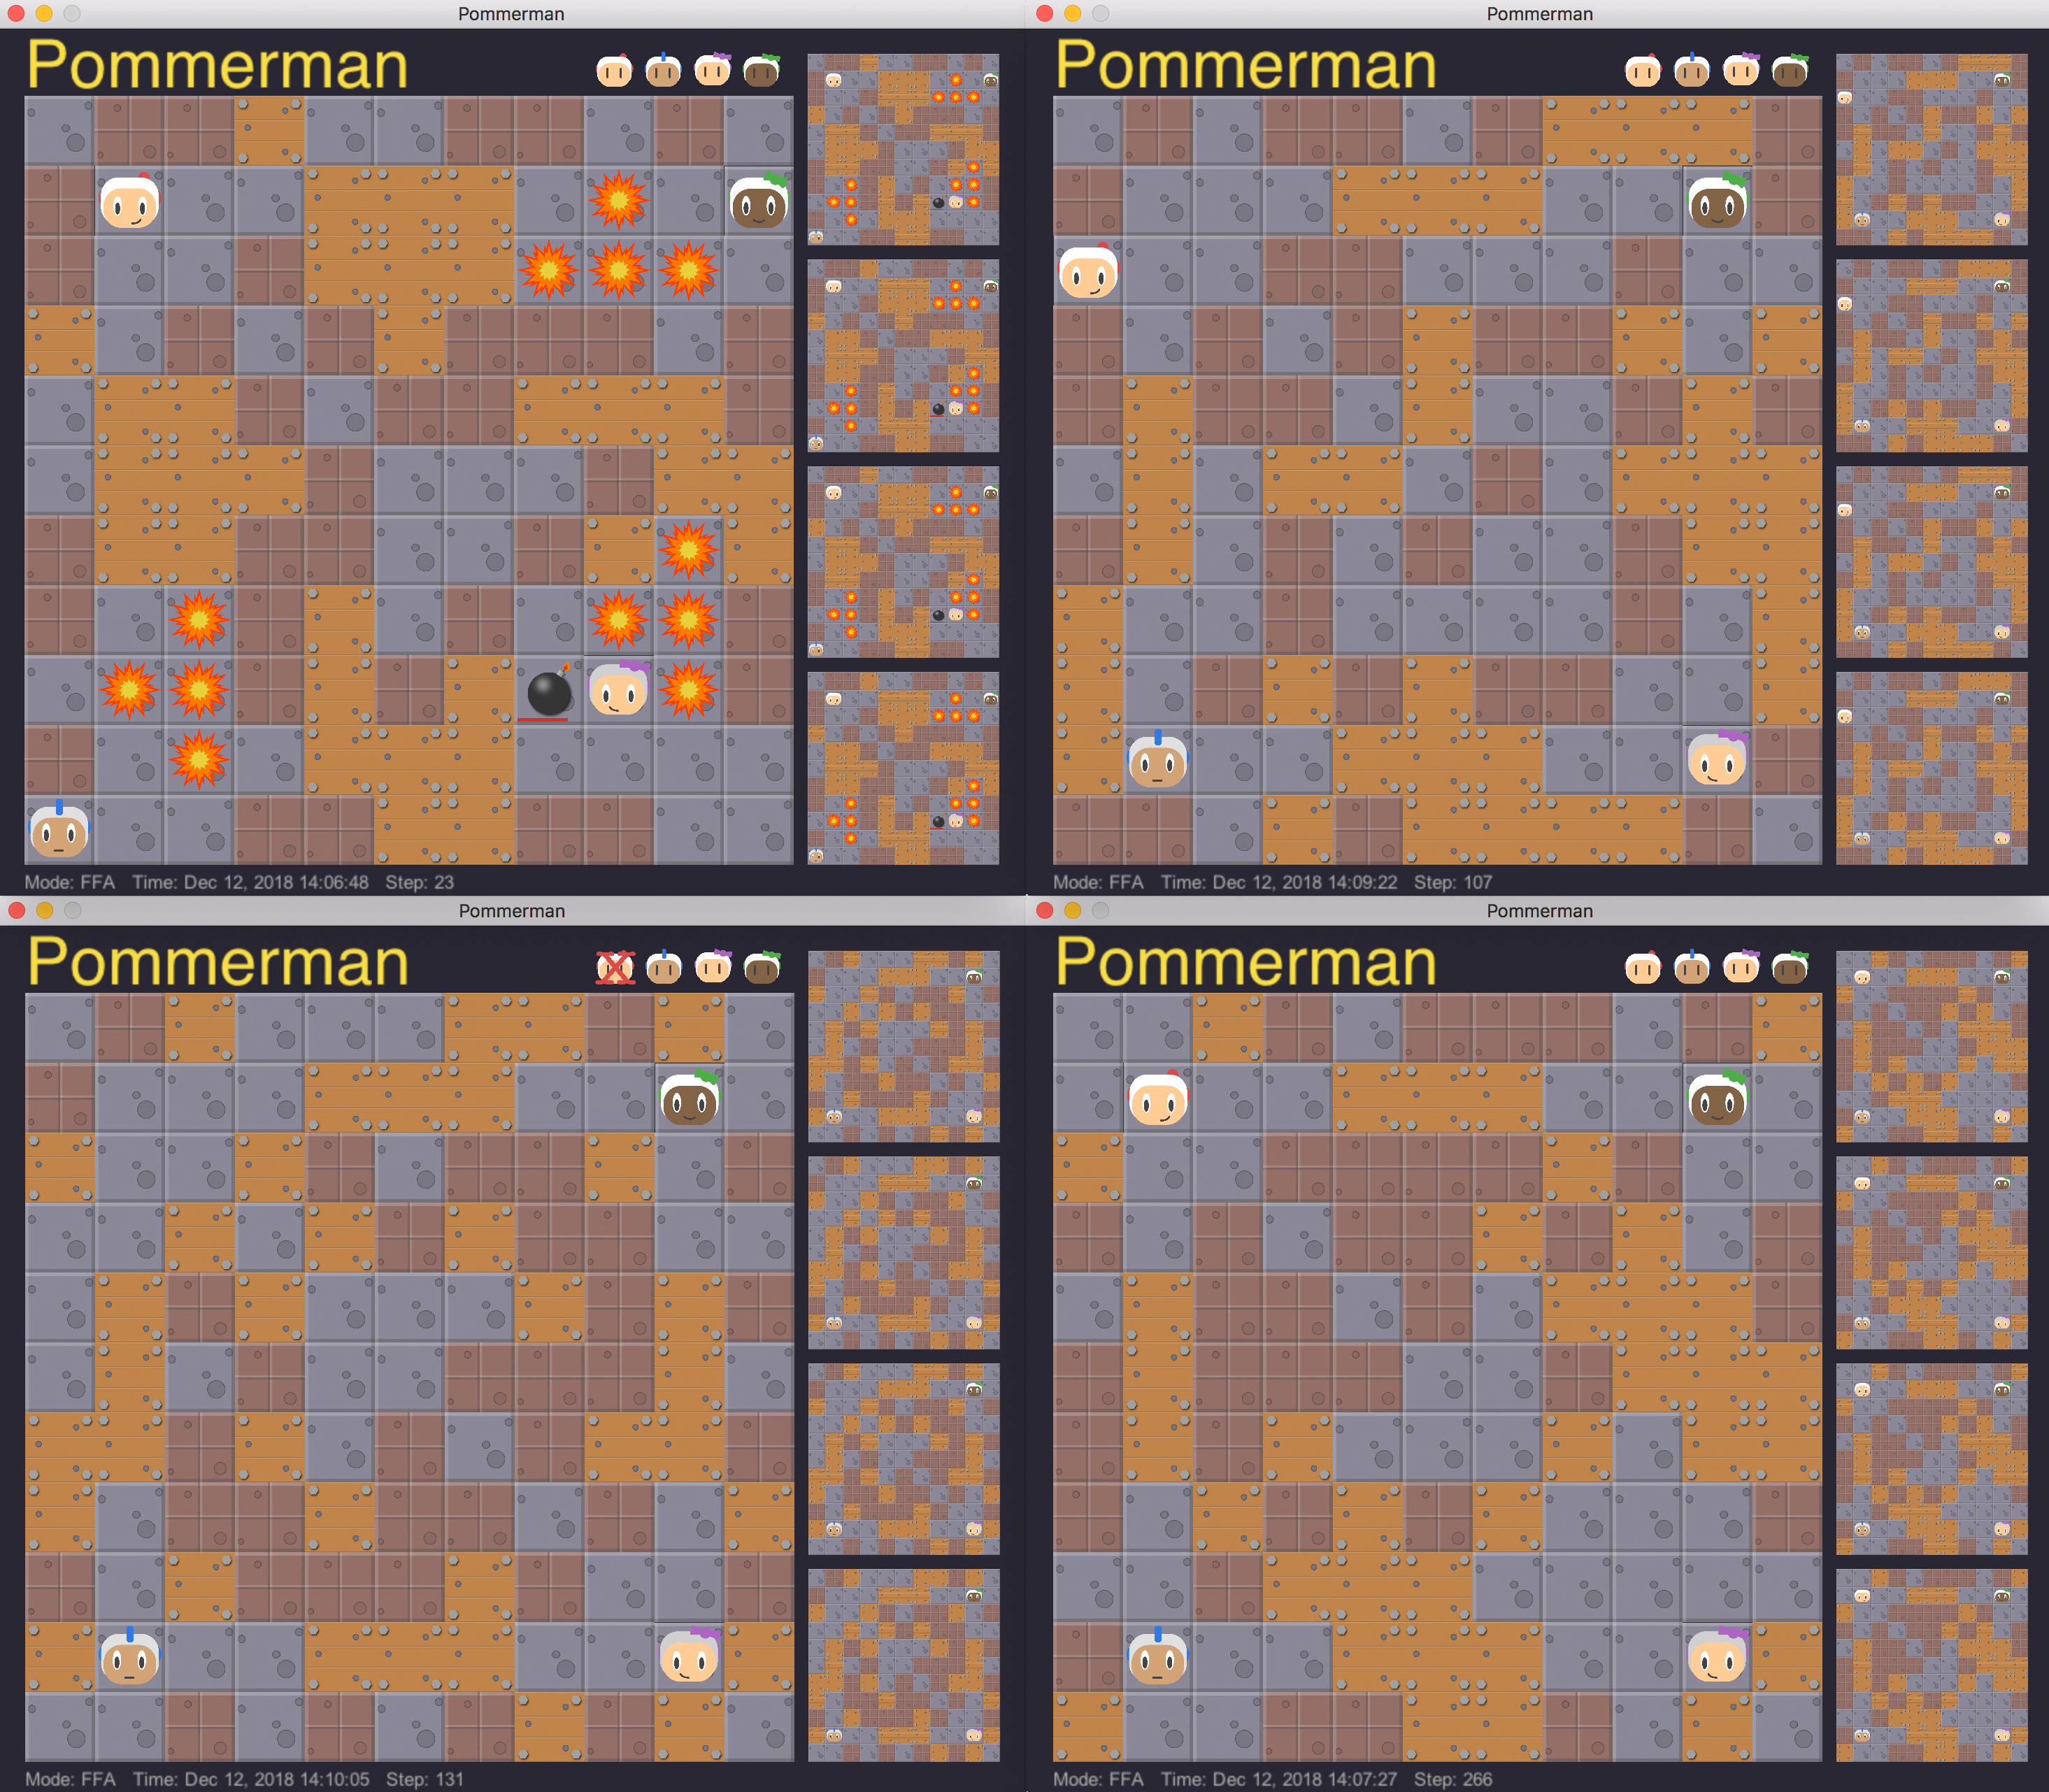
\includegraphics[width=0.7\linewidth]{docs/article/inputs/4pommerview.jpg}}
    \caption{Typical games of pommerman.}
    \label{fig:pomIntro}
\end{figure}